\documentclass[11pt,a4paper]{article}

\usepackage[utf8]{inputenc}
\usepackage[T1]{fontenc}
\usepackage[english]{babel}
\usepackage{amsmath}
\usepackage{amsfonts}
\usepackage{amssymb}
\usepackage{graphicx}
\usepackage[dvipsnames,table]{xcolor}
\usepackage{hyperref}
\usepackage{booktabs}
\usepackage{tabularx}
\usepackage{array}
\usepackage{enumitem}
\usepackage{geometry}
\usepackage{caption}
\usepackage{subcaption}
\usepackage{float}
\usepackage{tikz}
\usepackage{pgfplots}
\usetikzlibrary{arrows.meta, positioning, calc, fit}
\pgfplotsset{compat=1.18}

\geometry{a4paper, margin=1in}
\hypersetup{
    colorlinks=true,
    linkcolor=MidnightBlue,
    citecolor=ForestGreen,
    urlcolor=RoyalBlue
}

\setlist[itemize]{topsep=3pt, itemsep=2pt, leftmargin=*}
\renewcommand{\arraystretch}{1.18}
\newcolumntype{L}[1]{>{\raggedright\arraybackslash}p{#1}}
\newcolumntype{Y}{>{\raggedright\arraybackslash}X}

\definecolor{serverblue}{HTML}{1F4E79}
\definecolor{clientgreen}{HTML}{2E7D32}
\definecolor{accentorange}{HTML}{C75B12}
\definecolor{softgray}{HTML}{F5F7FA}

\title{\textbf{Evaluating Federated Image Classification under Non-IID Data:}\\
\large A Three-Node Comparative Study of FedAvg and FedProx}
\author{Author Name \\ \textit{Institution/Course Name} \\
\url{https://github.com/your-username/federated-learning-non-iid}}
\date{\today}

\begin{document}

\maketitle

\begin{abstract}
Federated Learning (FL) enables multiple distributed clients to train a shared machine learning model without centralizing their raw data. This design is attractive for privacy-sensitive and distributed environments, but it becomes unstable when clients own statistically different data distributions. In image classification, this non-independent and identically distributed (non-IID) condition can cause client drift: local models overfit to their own data shards and pull the global model in conflicting directions. This project proposes a controlled local simulation of a three-node federated learning system to compare Federated Averaging (FedAvg) against Federated Proximal (FedProx). FedAvg will be used as the baseline, while FedProx will be studied as a method for reducing instability through a proximal regularization term. The experiments will evaluate both algorithms across low, medium, and high non-IID partitions of MNIST, with CIFAR-10 considered as an extension. The study will measure not only classification performance, but also convergence behavior, inter-round variability, and sensitivity to the FedProx parameter $\mu$. The expected contribution is an empirical analysis of how statistical heterogeneity affects distributed AI training and whether FedProx provides a more stable learning process than FedAvg in a reproducible three-client environment.
\end{abstract}

\noindent\textbf{Keywords:} Federated Learning, Distributed AI, Non-IID Data, FedAvg, FedProx, Image Classification, Training Stability.

\section{Introduction and Research Problem}

Modern AI systems are increasingly trained across distributed data sources. In many realistic settings, such as hospitals, mobile devices, campuses, or edge sensors, data cannot be freely centralized because of privacy, ownership, bandwidth, or governance constraints. Federated Learning addresses this problem by allowing clients to train locally and send model updates to a central coordinator instead of sending raw data.

However, a core challenge appears when each client observes a different part of the world. For example, one hospital may contain mostly one patient group, while another may contain a different distribution of cases. In image classification, the same issue can be simulated when one node receives mostly digits 0--2, another receives 3--5, and a third receives 6--9. This non-IID distribution makes local optimization biased toward each client's data and can reduce the quality and stability of the global model.

\textbf{Research question.} To what extent does FedProx improve the performance and training stability of a classification model compared with FedAvg under different levels of non-IID data distribution among three local federated nodes?

This question clearly belongs to Artificial Intelligence because the main object of study is the behavior of machine learning algorithms for classification. At the same time, it connects with Distributed Systems because the model is trained through client-server coordination, communication rounds, local computation, model aggregation, and decentralized data ownership.

\subsection{Objectives}

\begin{itemize}
    \item Implement a reproducible three-client federated learning simulation using Python, PyTorch, and Flower.
    \item Generate controlled IID and non-IID data partitions for an image classification task.
    \item Compare FedAvg and FedProx across increasing levels of statistical heterogeneity.
    \item Measure final performance, convergence behavior, and training stability across communication rounds.
    \item Analyze the effect of the FedProx proximal coefficient $\mu$ on robustness and convergence.
\end{itemize}

\subsection{Hypotheses}

\begin{itemize}
    \item \textbf{H1:} Under low heterogeneity, FedAvg and FedProx will obtain similar classification performance.
    \item \textbf{H2:} As heterogeneity increases, FedProx will show lower inter-round variability than FedAvg.
    \item \textbf{H3:} Very large values of $\mu$ may overconstrain local learning, reducing the benefit of FedProx.
\end{itemize}

\section{Related Work}

Federated Learning was popularized by McMahan et al. through the FedAvg algorithm, which reduces communication costs by averaging locally trained model parameters across clients \cite{mcmahan2017communication}. FedAvg is effective when client data distributions are reasonably similar, but it can suffer from weight divergence and unstable convergence when data is highly heterogeneous.

Li et al. introduced FedProx to address heterogeneity in federated networks \cite{li2020federated}. FedProx modifies the local optimization objective by adding a proximal term that discourages each local model from moving too far away from the current global model. This makes it especially relevant for non-IID data, where each client may otherwise follow a strongly biased local direction. Hsu et al. further showed that non-identical data distributions can significantly affect federated visual classification \cite{hsu2019measuring}. Broader surveys, such as Kairouz et al., identify statistical heterogeneity, communication efficiency, and robustness as central open problems in FL \cite{kairouz2021advances}.

\begin{table}[H]
\centering
\caption{Positioning of the proposed project within related FL research.}
\begin{tabularx}{\textwidth}{L{2.4cm} L{3.0cm} L{3.0cm} Y}
\toprule
\textbf{Reference} & \textbf{Focus} & \textbf{Relevance} & \textbf{Connection to this project} \\
\midrule
McMahan et al. \cite{mcmahan2017communication} & Communication-efficient FL & Introduces FedAvg & FedAvg is used as the baseline algorithm. \\
Li et al. \cite{li2020federated} & FL under heterogeneity & Introduces FedProx & FedProx is the investigated method for improving stability. \\
Hsu et al. \cite{hsu2019measuring} & Non-IID visual classification & Shows effect of data skew & Motivates controlled non-IID image partitions. \\
Kairouz et al. \cite{kairouz2021advances} & FL survey and open problems & Identifies heterogeneity as key challenge & Frames the project as distributed AI research. \\
\bottomrule
\end{tabularx}
\end{table}

\section{Proposed System Architecture}

The project will be implemented as a local distributed simulation. Three clients will run as independent federated participants inside the same machine, each with its own local data partition and local training loop. A central federated server will coordinate communication rounds, distribute the current global model, collect model updates, perform aggregation, and evaluate the resulting global model.

\begin{figure}[!ht]
\centering
\resizebox{\textwidth}{!}{%
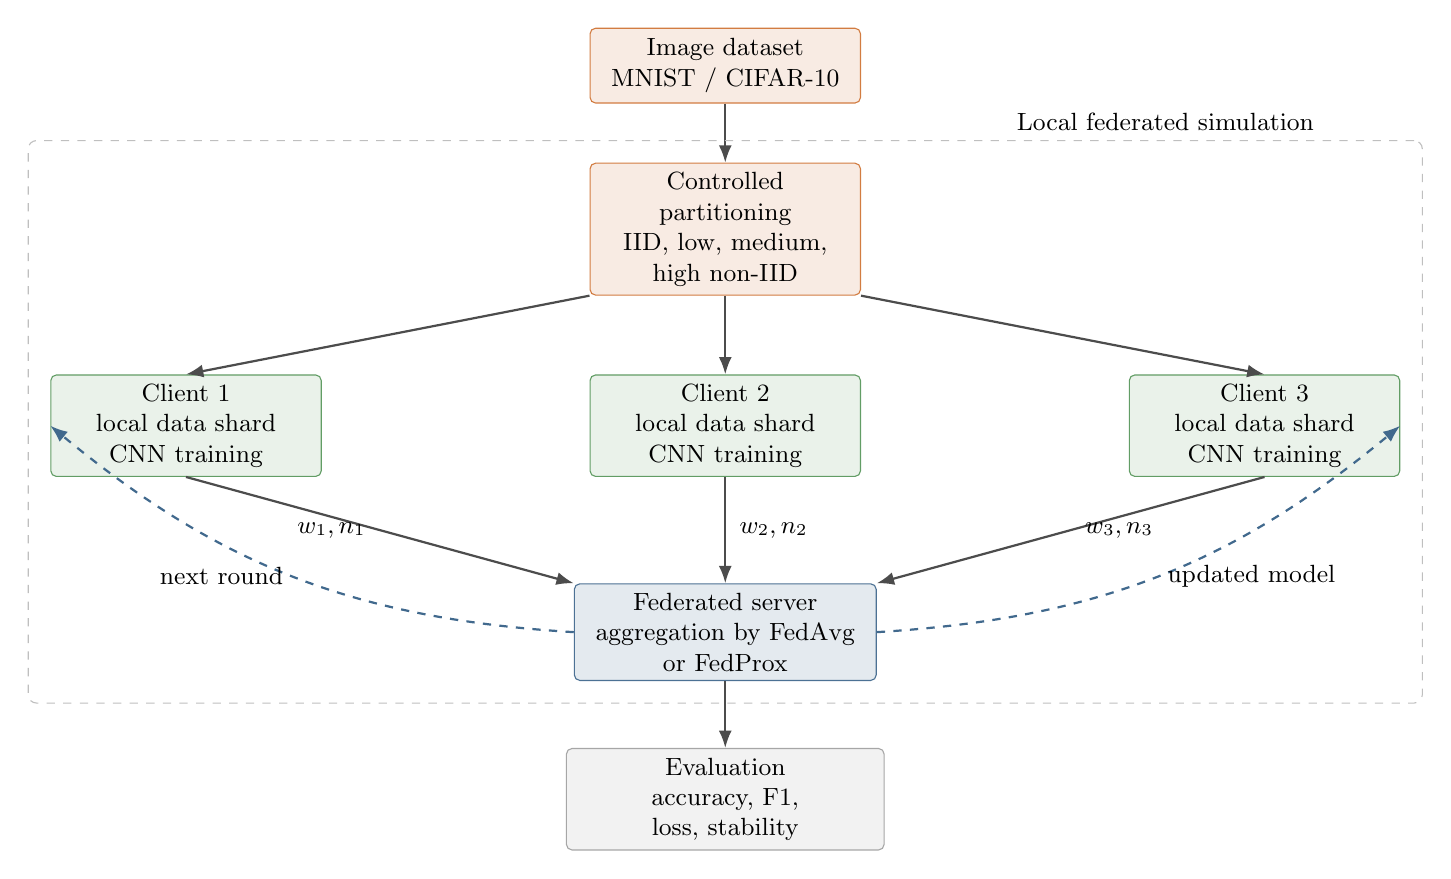
\begin{tikzpicture}[
    font=\small,
    block/.style={draw=black!55, rounded corners=2pt, align=center, minimum height=0.95cm, text width=3.2cm, fill=softgray},
    data/.style={block, fill=accentorange!12, draw=accentorange!80},
    client/.style={block, fill=clientgreen!10, draw=clientgreen!75},
    server/.style={block, fill=serverblue!12, draw=serverblue!80, text width=3.6cm},
    metric/.style={block, fill=gray!10, draw=gray!70, text width=3.8cm},
    arrow/.style={-{Latex[length=2.2mm]}, thick, draw=black!70},
    update/.style={-{Latex[length=2.2mm]}, thick, dashed, draw=serverblue!85}
]

\node[data] (dataset) {Image dataset\\MNIST / CIFAR-10};
\node[data, below=0.75cm of dataset] (partition) {Controlled partitioning\\IID, low, medium, high non-IID};

\node[client, below left=1.0cm and 3.4cm of partition] (c1) {Client 1\\local data shard\\CNN training};
\node[client, below=1.0cm of partition] (c2) {Client 2\\local data shard\\CNN training};
\node[client, below right=1.0cm and 3.4cm of partition] (c3) {Client 3\\local data shard\\CNN training};

\node[server, below=1.35cm of c2] (server) {Federated server\\aggregation by FedAvg\\or FedProx};
\node[metric, below=0.85cm of server] (eval) {Evaluation\\accuracy, F1, loss, stability};

\draw[arrow] (dataset) -- (partition);
\draw[arrow] (partition.south west) -- (c1.north);
\draw[arrow] (partition.south) -- (c2.north);
\draw[arrow] (partition.south east) -- (c3.north);

\draw[arrow] (c1.south) -- node[left, xshift=-0.05cm] {$w_1,n_1$} (server.north west);
\draw[arrow] (c2.south) -- node[right, xshift=0.05cm] {$w_2,n_2$} (server.north);
\draw[arrow] (c3.south) -- node[right, xshift=0.05cm] {$w_3,n_3$} (server.north east);
\draw[arrow] (server) -- (eval);

\draw[update] (server.west) to[bend left=18] node[left] {next round} (c1.west);
\draw[update] (server.east) to[bend right=18] node[right] {updated model} (c3.east);

\node[draw=black!25, dashed, rounded corners=3pt, fit=(partition)(c1)(c2)(c3)(server), inner sep=0.28cm, label={[font=\small]above right:Local federated simulation}] {};
\end{tikzpicture}
}
\caption{Proposed three-client federated learning architecture. Raw data remains local to each client; only model parameters or updates are communicated to the server.}
\label{fig:architecture}
\end{figure}

This design keeps the project feasible while still preserving the essential distributed-system properties of FL: multiple participants, decentralized data, iterative communication, server-side coordination, and global aggregation.

\section{Methodology}

\subsection{Dataset and Preprocessing}

The initial dataset will be MNIST because it allows fast experimentation with a lightweight convolutional neural network (CNN). CIFAR-10 will be considered as an extension if the MNIST pipeline is completed early. The dataset will be partitioned among three clients using controlled heterogeneity levels:

\begin{itemize}
    \item \textbf{IID baseline:} each client receives a balanced random sample of all labels.
    \item \textbf{Low non-IID:} each client receives all labels, but with mild label imbalance.
    \item \textbf{Medium non-IID:} each client is biased toward a subset of labels while still containing some examples from other labels.
    \item \textbf{High non-IID:} each client primarily receives disjoint label groups, such as digits 0--2, 3--5, and 6--9.
\end{itemize}

The non-IID partitions may be produced using label-skew rules or a Dirichlet distribution. The degree of heterogeneity will be treated as an independent variable rather than an accidental property of the dataset.

\subsection{Algorithms}

The baseline is \textbf{FedAvg}. At communication round $t$, each client $k$ trains locally and returns parameters $w_k^{(t+1)}$. The server computes a weighted average:

\[
w^{(t+1)} = \sum_{k=1}^{K} \frac{n_k}{n} w_k^{(t+1)}
\]

where $K$ is the number of clients and $n_k$ is the number of training examples on client $k$. The total number of training examples is:

\[
n = \sum_{k=1}^{K} n_k
\]

The investigated method is \textbf{FedProx}. It modifies each local objective by adding a proximal penalty:

\[
\min_w F_k(w) + \frac{\mu}{2}\left\|w - w^{(t)}\right\|_2^2
\]

The proximal term discourages local models from drifting too far from the current global model $w^{(t)}$. The coefficient $\mu$ controls the strength of this constraint. The planned values are:

\[
\mu \in \{0.001, 0.01, 0.1, 1.0\}
\]

\subsection{Experimental Design}

The project will compare the algorithms across a matrix of data heterogeneity levels. FedAvg is evaluated once per heterogeneity level, while FedProx is evaluated with multiple values of $\mu$.

\begin{table}[H]
\centering
\caption{Planned experimental matrix. Each configuration will be evaluated across multiple communication rounds.}
\begin{tabularx}{\textwidth}{L{2.6cm} L{2.4cm} L{2.4cm} Y}
\toprule
\textbf{Heterogeneity} & \textbf{Algorithm} & \textbf{Parameter} & \textbf{Purpose} \\
\midrule
IID & FedAvg & -- & Verify the baseline pipeline under balanced data. \\
Low / Medium / High & FedAvg & -- & Measure how the baseline degrades as client data becomes skewed. \\
Low / Medium / High & FedProx & $\mu=0.001$ & Test a weak proximal constraint. \\
Low / Medium / High & FedProx & $\mu=0.01$ & Test a moderate proximal constraint. \\
Low / Medium / High & FedProx & $\mu=0.1$ & Test a stronger proximal constraint. \\
Low / Medium / High & FedProx & $\mu=1.0$ & Detect whether excessive constraint harms learning. \\
\bottomrule
\end{tabularx}
\end{table}

Whenever time permits, each configuration will be repeated with different random seeds to reduce the risk that conclusions depend on one specific data partition.

\section{Benchmark and Evaluation Metrics}

FedAvg will serve as the benchmark because it is the standard baseline in many FL experiments. FedProx will be compared against it using both final-performance metrics and training-dynamics metrics.

\begin{table}[H]
\centering
\caption{Evaluation variables and their role in the study.}
\begin{tabularx}{\textwidth}{L{3.1cm} L{3.6cm} Y}
\toprule
\textbf{Metric} & \textbf{What it measures} & \textbf{Why it matters} \\
\midrule
Accuracy & Correct predictions over the test set & Main classification performance metric. \\
Precision, Recall, F1-score & Class-level prediction quality & Useful when label distributions become skewed. \\
Global loss & Optimization progress & Shows whether the model is converging or oscillating. \\
Rounds to target accuracy & Convergence speed & Indicates communication efficiency. \\
Inter-round variability & Stability of learning & Captures whether performance fluctuates across rounds. \\
\bottomrule
\end{tabularx}
\end{table}

Training stability will be operationalized using the standard deviation of the change in global accuracy between communication rounds:

\[
S_{\Delta acc} =
\sqrt{
\frac{1}{R-1}\sum_{r=2}^{R}
\left(\Delta acc_r - \overline{\Delta acc}\right)^2
},
\qquad
\Delta acc_r = acc_r - acc_{r-1}
\]

A lower value of $S_{\Delta acc}$ indicates smoother training. This makes the term "stability" measurable instead of only descriptive.

\section{Preliminary Results}

The current implementation already contains a basic Flower simulation with three clients, a PyTorch CNN, MNIST loading, IID partitioning, local training, and FedAvg aggregation. This first stage is not meant to prove that FedAvg is superior or inferior; it verifies that the pipeline can run end-to-end before adding non-IID partitions and FedProx.

\begin{table}[H]
\centering
\caption{Preliminary smoke-test results: FedAvg on MNIST with IID partitioning.}
\begin{tabular}{ccc}
\toprule
\textbf{Round} & \textbf{Global Accuracy} & \textbf{Global Loss} \\
\midrule
1 & 0.82 & 0.54 \\
3 & 0.91 & 0.23 \\
5 & 0.94 & 0.15 \\
\bottomrule
\end{tabular}
\end{table}

\begin{figure}[H]
\centering
\begin{subfigure}[t]{0.48\textwidth}
\centering
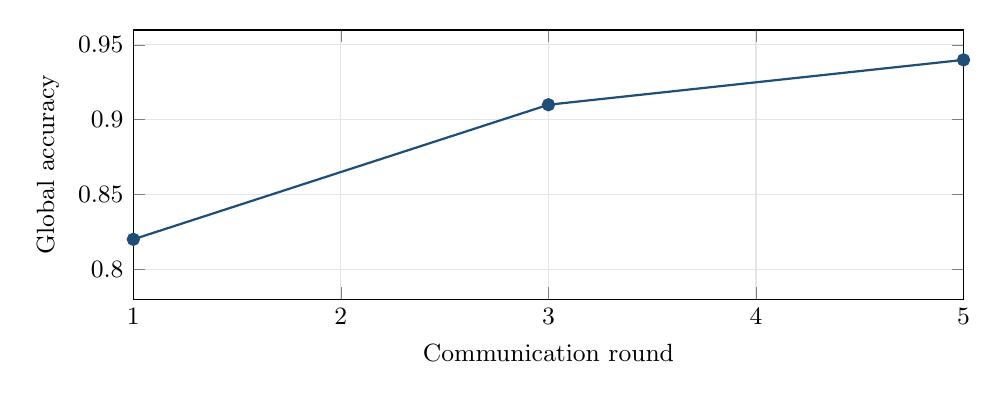
\begin{tikzpicture}
\begin{axis}[
    width=\linewidth,
    height=5cm,
    xlabel={Communication round},
    ylabel={Global accuracy},
    xmin=1, xmax=5,
    ymin=0.78, ymax=0.96,
    xtick={1,2,3,4,5},
    ytick={0.80,0.85,0.90,0.95},
    grid=both,
    grid style={gray!20},
    tick label style={font=\small},
    label style={font=\small}
]
\addplot[color=serverblue, mark=*, thick] coordinates {(1,0.82) (3,0.91) (5,0.94)};
\end{axis}
\end{tikzpicture}
\caption{Accuracy trend}
\end{subfigure}
\hfill
\begin{subfigure}[t]{0.48\textwidth}
\centering
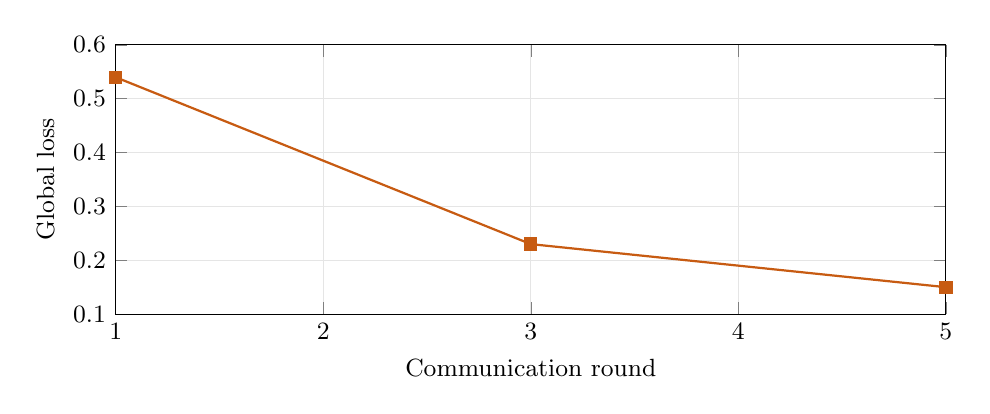
\begin{tikzpicture}
\begin{axis}[
    width=\linewidth,
    height=5cm,
    xlabel={Communication round},
    ylabel={Global loss},
    xmin=1, xmax=5,
    ymin=0.10, ymax=0.60,
    xtick={1,2,3,4,5},
    ytick={0.10,0.20,0.30,0.40,0.50,0.60},
    grid=both,
    grid style={gray!20},
    tick label style={font=\small},
    label style={font=\small}
]
\addplot[color=accentorange, mark=square*, thick] coordinates {(1,0.54) (3,0.23) (5,0.15)};
\end{axis}
\end{tikzpicture}
\caption{Loss trend}
\end{subfigure}
\caption{Preliminary FedAvg/IID trends from the initial local simulation. These plots are used as evidence that the experimental workflow is functional, not as final comparative results.}
\label{fig:prelim}
\end{figure}

The next implementation step is to replace the IID splitter with controlled non-IID partitioning and add the FedProx local objective. After that, the full experimental matrix can be executed.

\section{Expected Results and Discussion}

The expected pattern is that FedAvg will perform well under IID or low non-IID settings, but its learning curve may become less stable as the clients become more specialized. In high non-IID settings, local models are expected to move in conflicting directions, producing slower convergence or stronger accuracy oscillations. FedProx is expected to reduce this effect by limiting local drift from the global model.

The most important result will not be a single final accuracy value. Instead, the study will analyze whether the advantage of FedProx grows as heterogeneity increases. If FedProx improves final accuracy but also requires careful tuning of $\mu$, the project will discuss that trade-off. If FedProx does not outperform FedAvg under some conditions, that will also be meaningful because it will define when the added proximal constraint is unnecessary.

\section{Reproducibility and Deliverables}

All experiments will be designed to be reproducible. The repository will include the source code, dependency list, dataset download instructions, partitioning settings, random seeds, experiment logs, and generated plots.

\begin{itemize}
    \item \textbf{Code:} Python implementation using PyTorch and Flower.
    \item \textbf{Data:} MNIST downloaded through torchvision; CIFAR-10 as optional extension.
    \item \textbf{Configurations:} heterogeneity level, algorithm, $\mu$, number of rounds, batch size, local epochs, and random seed.
    \item \textbf{Outputs:} accuracy/loss curves, comparison tables, stability metrics, and final discussion.
\end{itemize}

\noindent\textbf{GitHub Repository:} \url{https://github.com/your-username/federated-learning-non-iid}

\section{Limitations}

This proposal uses a local simulation rather than physically separate machines. This is appropriate for isolating the AI research question, but it does not fully measure real network latency, packet loss, or hardware heterogeneity. The distributed-systems extension may later execute the same server and clients as separate processes or machines. Another limitation is that MNIST is relatively simple; therefore, CIFAR-10 may be used as a secondary dataset if time allows.

\begin{thebibliography}{99}

\bibitem{mcmahan2017communication}
McMahan, B., Moore, E., Ramage, D., Hampson, S., \& y Arcas, B. A. (2017).
Communication-efficient learning of deep networks from decentralized data.
In \textit{Artificial Intelligence and Statistics} (pp. 1273--1282). PMLR.

\bibitem{li2020federated}
Li, T., Sahu, A. K., Zaheer, M., Sanjabi, M., Talwalkar, A., \& Smith, V. (2020).
Federated optimization in heterogeneous networks.
\textit{Proceedings of Machine Learning and Systems}, 2, 429--450.

\bibitem{hsu2019measuring}
Hsu, T.-M. H., Qi, H., \& Brown, M. (2019).
Measuring the effects of non-identical data distribution for federated visual classification.
\textit{arXiv preprint arXiv:1909.06335}.

\bibitem{kairouz2021advances}
Kairouz, P., McMahan, H. B., Avent, B., Bellet, A., Bennis, M., Bhagoji, A. N., Bonawitz, K., Charles, Z., Cormode, G., Cummings, R., et al. (2021).
Advances and open problems in federated learning.
\textit{Foundations and Trends in Machine Learning}, 14(1--2), 1--210.

\end{thebibliography}

\end{document}
